\section{Results}

\subsection{Neural network classifier}
SIFT descriptors were extracted from each image, with a maximum of 100 descriptors per image.
A random subset of 100 of the files containing these descriptors was used for the clustering step in the bag-of-words process, in which the descriptors were mapped onto 100 clusters.
This number of clusters was empirically found to provide a good trade-off between accuracy and computation time.
A subset of all SIFT descriptors was used to ensure clustering completed within a reasonable time span.
The neural network, containing 100 hidden nodes, was run for 1,000 epochs with a learn rate of 0.1 and no regularisation.
Classifications were considered correct if the ground truth class appeared in the top 5 results.
Using this metric, the network's classification accuracy was 77.78\%.

\subsection{KNN classifier}
As with the neural network classifier, a maximum of 100 SIFT descriptors were extracted from each image.
Once again a random subset of 100 of the files containing these descriptors was used for creating the 100 clusters of the visual bag-of-words.
The classifier was run on the test data for values of $K$ ranging from 1 to 100.
The highest accuracy of 60.9\% was achieved with $K = 32$.

Classifications were considered correct if the ground truth class appeared in the top $T$ results.
Figure \vref{fig:knnresults} shows the accuracy of the KNN classifier at various values of $T$, with $K$ ranging from 1 to 100.
Performance remains more or less steady once $K$ is above 10.
The marginal gain in accuracy for larger values of $T$ decreases rapidly with $T$ --- the step from $T=4$ to $T=5$ only improves the classifier's performance very slightly.


\begin{figure}[htb]
	\centering
	% Created by tikzDevice version 0.8.1 on 2016-02-05 20:58:22
% !TEX encoding = UTF-8 Unicode
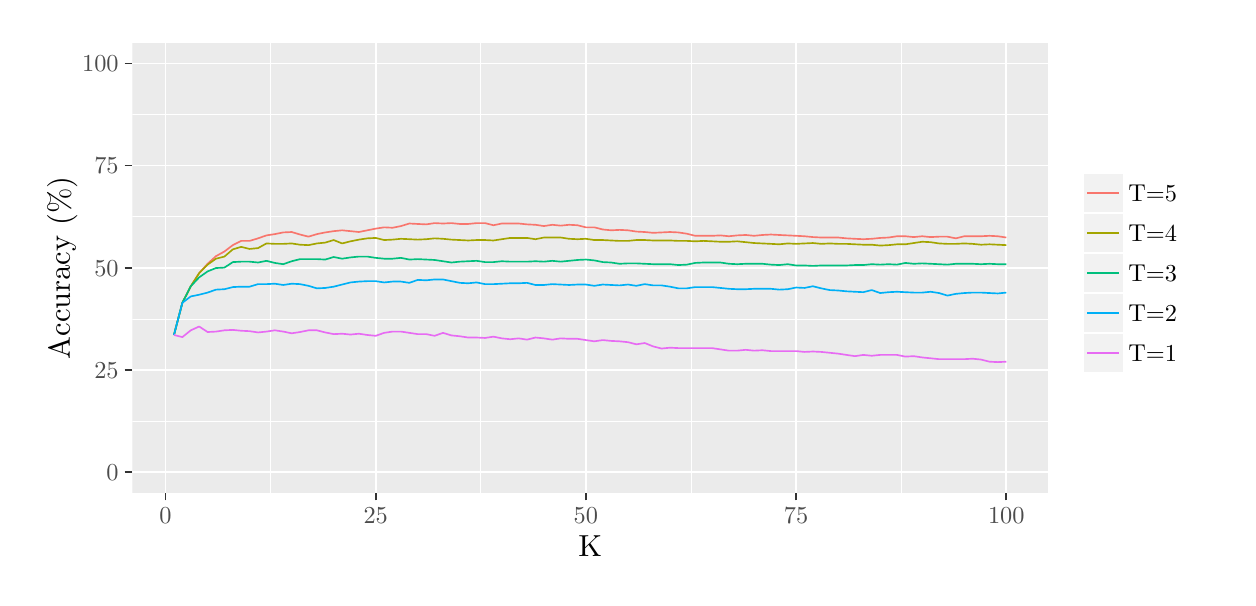
\begin{tikzpicture}[x=1pt,y=1pt]
\definecolor{fillColor}{RGB}{255,255,255}
\path[use as bounding box,fill=fillColor,fill opacity=0.00] (0,0) rectangle (433.62,198.74);
\begin{scope}
\path[clip] (  0.00,  0.00) rectangle (433.62,198.74);
\definecolor{drawColor}{RGB}{255,255,255}
\definecolor{fillColor}{RGB}{255,255,255}

\path[draw=drawColor,line width= 0.6pt,line join=round,line cap=round,fill=fillColor] (  0.00,  0.00) rectangle (433.62,198.74);
\end{scope}
\begin{scope}
\path[clip] ( 37.82, 30.69) rectangle (368.66,193.24);
\definecolor{fillColor}{gray}{0.92}

\path[fill=fillColor] ( 37.82, 30.69) rectangle (368.66,193.24);
\definecolor{drawColor}{RGB}{255,255,255}

\path[draw=drawColor,line width= 0.3pt,line join=round] ( 37.82, 56.55) --
	(368.66, 56.55);

\path[draw=drawColor,line width= 0.3pt,line join=round] ( 37.82, 93.49) --
	(368.66, 93.49);

\path[draw=drawColor,line width= 0.3pt,line join=round] ( 37.82,130.44) --
	(368.66,130.44);

\path[draw=drawColor,line width= 0.3pt,line join=round] ( 37.82,167.38) --
	(368.66,167.38);

\path[draw=drawColor,line width= 0.3pt,line join=round] ( 87.80, 30.69) --
	( 87.80,193.24);

\path[draw=drawColor,line width= 0.3pt,line join=round] (163.75, 30.69) --
	(163.75,193.24);

\path[draw=drawColor,line width= 0.3pt,line join=round] (239.69, 30.69) --
	(239.69,193.24);

\path[draw=drawColor,line width= 0.3pt,line join=round] (315.64, 30.69) --
	(315.64,193.24);

\path[draw=drawColor,line width= 0.6pt,line join=round] ( 37.82, 38.08) --
	(368.66, 38.08);

\path[draw=drawColor,line width= 0.6pt,line join=round] ( 37.82, 75.02) --
	(368.66, 75.02);

\path[draw=drawColor,line width= 0.6pt,line join=round] ( 37.82,111.96) --
	(368.66,111.96);

\path[draw=drawColor,line width= 0.6pt,line join=round] ( 37.82,148.91) --
	(368.66,148.91);

\path[draw=drawColor,line width= 0.6pt,line join=round] ( 37.82,185.85) --
	(368.66,185.85);

\path[draw=drawColor,line width= 0.6pt,line join=round] ( 49.82, 30.69) --
	( 49.82,193.24);

\path[draw=drawColor,line width= 0.6pt,line join=round] (125.77, 30.69) --
	(125.77,193.24);

\path[draw=drawColor,line width= 0.6pt,line join=round] (201.72, 30.69) --
	(201.72,193.24);

\path[draw=drawColor,line width= 0.6pt,line join=round] (277.67, 30.69) --
	(277.67,193.24);

\path[draw=drawColor,line width= 0.6pt,line join=round] (353.62, 30.69) --
	(353.62,193.24);
\definecolor{drawColor}{RGB}{248,118,109}

\path[draw=drawColor,line width= 0.6pt,line join=round] ( 52.86, 87.69) --
	( 55.90, 99.33) --
	( 58.94,105.30) --
	( 61.97,110.05) --
	( 65.01,113.42) --
	( 68.05,116.18) --
	( 71.09,117.86) --
	( 74.13,120.16) --
	( 77.16,121.69) --
	( 80.20,121.69) --
	( 83.24,122.61) --
	( 86.28,123.68) --
	( 89.32,124.14) --
	( 92.35,124.75) --
	( 95.39,124.90) --
	( 98.43,123.99) --
	(101.47,123.22) --
	(104.51,124.14) --
	(107.54,124.75) --
	(110.58,125.21) --
	(113.62,125.52) --
	(116.66,125.21) --
	(119.70,124.90) --
	(122.73,125.52) --
	(125.77,126.13) --
	(128.81,126.59) --
	(131.85,126.44) --
	(134.89,127.05) --
	(137.92,127.97) --
	(140.96,127.81) --
	(144.00,127.66) --
	(147.04,128.12) --
	(150.08,127.97) --
	(153.11,128.12) --
	(156.15,127.81) --
	(159.19,127.81) --
	(162.23,128.12) --
	(165.26,128.12) --
	(168.30,127.35) --
	(171.34,127.97) --
	(174.38,127.97) --
	(177.42,127.97) --
	(180.45,127.66) --
	(183.49,127.51) --
	(186.53,127.05) --
	(189.57,127.51) --
	(192.61,127.20) --
	(195.64,127.51) --
	(198.68,127.35) --
	(201.72,126.59) --
	(204.76,126.59) --
	(207.80,125.82) --
	(210.83,125.52) --
	(213.87,125.67) --
	(216.91,125.52) --
	(219.95,125.06) --
	(222.99,124.90) --
	(226.02,124.60) --
	(229.06,124.75) --
	(232.10,124.90) --
	(235.14,124.75) --
	(238.18,124.29) --
	(241.21,123.53) --
	(244.25,123.53) --
	(247.29,123.53) --
	(250.33,123.68) --
	(253.37,123.37) --
	(256.40,123.68) --
	(259.44,123.83) --
	(262.48,123.53) --
	(265.52,123.83) --
	(268.56,123.99) --
	(271.59,123.83) --
	(274.63,123.68) --
	(277.67,123.53) --
	(280.71,123.37) --
	(283.75,123.07) --
	(286.78,122.91) --
	(289.82,122.91) --
	(292.86,122.91) --
	(295.90,122.61) --
	(298.93,122.45) --
	(301.97,122.30) --
	(305.01,122.45) --
	(308.05,122.76) --
	(311.09,122.91) --
	(314.12,123.37) --
	(317.16,123.37) --
	(320.20,123.07) --
	(323.24,123.37) --
	(326.28,123.07) --
	(329.31,123.22) --
	(332.35,123.22) --
	(335.39,122.61) --
	(338.43,123.37) --
	(341.47,123.37) --
	(344.50,123.37) --
	(347.54,123.53) --
	(350.58,123.37) --
	(353.62,122.91);
\definecolor{drawColor}{RGB}{163,165,0}

\path[draw=drawColor,line width= 0.6pt,line join=round] ( 52.86, 87.69) --
	( 55.90, 99.33) --
	( 58.94,105.30) --
	( 61.97,110.05) --
	( 65.01,113.11) --
	( 68.05,115.26) --
	( 71.09,116.02) --
	( 74.13,118.63) --
	( 77.16,119.54) --
	( 80.20,118.78) --
	( 83.24,119.09) --
	( 86.28,120.77) --
	( 89.32,120.62) --
	( 92.35,120.62) --
	( 95.39,120.77) --
	( 98.43,120.31) --
	(101.47,120.16) --
	(104.51,120.77) --
	(107.54,121.08) --
	(110.58,122.00) --
	(113.62,120.77) --
	(116.66,121.54) --
	(119.70,122.15) --
	(122.73,122.61) --
	(125.77,122.76) --
	(128.81,122.00) --
	(131.85,122.15) --
	(134.89,122.45) --
	(137.92,122.30) --
	(140.96,122.15) --
	(144.00,122.30) --
	(147.04,122.61) --
	(150.08,122.45) --
	(153.11,122.15) --
	(156.15,122.00) --
	(159.19,121.84) --
	(162.23,122.00) --
	(165.26,122.00) --
	(168.30,121.84) --
	(171.34,122.30) --
	(174.38,122.76) --
	(177.42,122.76) --
	(180.45,122.76) --
	(183.49,122.30) --
	(186.53,122.91) --
	(189.57,122.91) --
	(192.61,122.91) --
	(195.64,122.45) --
	(198.68,122.30) --
	(201.72,122.45) --
	(204.76,122.00) --
	(207.80,122.00) --
	(210.83,121.84) --
	(213.87,121.69) --
	(216.91,121.69) --
	(219.95,122.00) --
	(222.99,122.00) --
	(226.02,121.84) --
	(229.06,121.84) --
	(232.10,121.84) --
	(235.14,121.69) --
	(238.18,121.69) --
	(241.21,121.54) --
	(244.25,121.69) --
	(247.29,121.54) --
	(250.33,121.38) --
	(253.37,121.38) --
	(256.40,121.54) --
	(259.44,121.23) --
	(262.48,120.92) --
	(265.52,120.77) --
	(268.56,120.62) --
	(271.59,120.46) --
	(274.63,120.77) --
	(277.67,120.62) --
	(280.71,120.77) --
	(283.75,120.92) --
	(286.78,120.62) --
	(289.82,120.77) --
	(292.86,120.62) --
	(295.90,120.62) --
	(298.93,120.46) --
	(301.97,120.31) --
	(305.01,120.31) --
	(308.05,120.00) --
	(311.09,120.16) --
	(314.12,120.46) --
	(317.16,120.46) --
	(320.20,120.92) --
	(323.24,121.38) --
	(326.28,121.23) --
	(329.31,120.77) --
	(332.35,120.62) --
	(335.39,120.62) --
	(338.43,120.77) --
	(341.47,120.62) --
	(344.50,120.31) --
	(347.54,120.46) --
	(350.58,120.31) --
	(353.62,120.16);
\definecolor{drawColor}{RGB}{0,191,125}

\path[draw=drawColor,line width= 0.6pt,line join=round] ( 52.86, 87.69) --
	( 55.90, 99.33) --
	( 58.94,105.30) --
	( 61.97,108.52) --
	( 65.01,110.66) --
	( 68.05,111.89) --
	( 71.09,112.04) --
	( 74.13,114.03) --
	( 77.16,114.19) --
	( 80.20,114.19) --
	( 83.24,113.88) --
	( 86.28,114.49) --
	( 89.32,113.73) --
	( 92.35,113.27) --
	( 95.39,114.34) --
	( 98.43,115.10) --
	(101.47,115.10) --
	(104.51,115.10) --
	(107.54,114.95) --
	(110.58,115.87) --
	(113.62,115.26) --
	(116.66,115.72) --
	(119.70,116.02) --
	(122.73,116.02) --
	(125.77,115.56) --
	(128.81,115.26) --
	(131.85,115.26) --
	(134.89,115.56) --
	(137.92,114.95) --
	(140.96,115.10) --
	(144.00,114.95) --
	(147.04,114.80) --
	(150.08,114.34) --
	(153.11,113.88) --
	(156.15,114.19) --
	(159.19,114.34) --
	(162.23,114.49) --
	(165.26,114.03) --
	(168.30,114.03) --
	(171.34,114.34) --
	(174.38,114.19) --
	(177.42,114.19) --
	(180.45,114.19) --
	(183.49,114.34) --
	(186.53,114.19) --
	(189.57,114.49) --
	(192.61,114.19) --
	(195.64,114.49) --
	(198.68,114.80) --
	(201.72,114.95) --
	(204.76,114.64) --
	(207.80,114.03) --
	(210.83,113.88) --
	(213.87,113.42) --
	(216.91,113.57) --
	(219.95,113.57) --
	(222.99,113.42) --
	(226.02,113.27) --
	(229.06,113.27) --
	(232.10,113.27) --
	(235.14,112.96) --
	(238.18,113.11) --
	(241.21,113.73) --
	(244.25,113.88) --
	(247.29,113.88) --
	(250.33,113.88) --
	(253.37,113.42) --
	(256.40,113.27) --
	(259.44,113.42) --
	(262.48,113.42) --
	(265.52,113.42) --
	(268.56,113.11) --
	(271.59,112.96) --
	(274.63,113.27) --
	(277.67,112.81) --
	(280.71,112.81) --
	(283.75,112.65) --
	(286.78,112.81) --
	(289.82,112.81) --
	(292.86,112.81) --
	(295.90,112.81) --
	(298.93,112.96) --
	(301.97,112.96) --
	(305.01,113.27) --
	(308.05,113.11) --
	(311.09,113.27) --
	(314.12,113.11) --
	(317.16,113.73) --
	(320.20,113.42) --
	(323.24,113.57) --
	(326.28,113.42) --
	(329.31,113.27) --
	(332.35,113.11) --
	(335.39,113.42) --
	(338.43,113.42) --
	(341.47,113.42) --
	(344.50,113.27) --
	(347.54,113.42) --
	(350.58,113.27) --
	(353.62,113.27);
\definecolor{drawColor}{RGB}{0,176,246}

\path[draw=drawColor,line width= 0.6pt,line join=round] ( 52.86, 87.69) --
	( 55.90, 99.33) --
	( 58.94,101.63) --
	( 61.97,102.24) --
	( 65.01,103.01) --
	( 68.05,104.08) --
	( 71.09,104.23) --
	( 74.13,105.00) --
	( 77.16,105.15) --
	( 80.20,105.15) --
	( 83.24,106.07) --
	( 86.28,106.07) --
	( 89.32,106.22) --
	( 92.35,105.76) --
	( 95.39,106.22) --
	( 98.43,106.07) --
	(101.47,105.46) --
	(104.51,104.54) --
	(107.54,104.69) --
	(110.58,105.15) --
	(113.62,105.92) --
	(116.66,106.68) --
	(119.70,106.99) --
	(122.73,107.14) --
	(125.77,107.14) --
	(128.81,106.68) --
	(131.85,106.99) --
	(134.89,106.99) --
	(137.92,106.53) --
	(140.96,107.60) --
	(144.00,107.45) --
	(147.04,107.75) --
	(150.08,107.75) --
	(153.11,107.14) --
	(156.15,106.53) --
	(159.19,106.38) --
	(162.23,106.68) --
	(165.26,106.07) --
	(168.30,106.07) --
	(171.34,106.22) --
	(174.38,106.38) --
	(177.42,106.38) --
	(180.45,106.53) --
	(183.49,105.76) --
	(186.53,105.76) --
	(189.57,106.07) --
	(192.61,105.92) --
	(195.64,105.76) --
	(198.68,105.92) --
	(201.72,105.92) --
	(204.76,105.46) --
	(207.80,105.92) --
	(210.83,105.76) --
	(213.87,105.61) --
	(216.91,105.92) --
	(219.95,105.46) --
	(222.99,106.07) --
	(226.02,105.61) --
	(229.06,105.61) --
	(232.10,105.15) --
	(235.14,104.54) --
	(238.18,104.54) --
	(241.21,105.00) --
	(244.25,105.00) --
	(247.29,105.00) --
	(250.33,104.69) --
	(253.37,104.38) --
	(256.40,104.23) --
	(259.44,104.23) --
	(262.48,104.38) --
	(265.52,104.38) --
	(268.56,104.38) --
	(271.59,104.08) --
	(274.63,104.23) --
	(277.67,104.84) --
	(280.71,104.69) --
	(283.75,105.30) --
	(286.78,104.54) --
	(289.82,103.92) --
	(292.86,103.77) --
	(295.90,103.47) --
	(298.93,103.31) --
	(301.97,103.16) --
	(305.01,103.92) --
	(308.05,102.85) --
	(311.09,103.16) --
	(314.12,103.31) --
	(317.16,103.16) --
	(320.20,103.01) --
	(323.24,103.01) --
	(326.28,103.31) --
	(329.31,102.85) --
	(332.35,101.93) --
	(335.39,102.55) --
	(338.43,102.85) --
	(341.47,103.01) --
	(344.50,103.01) --
	(347.54,102.85) --
	(350.58,102.70) --
	(353.62,103.01);
\definecolor{drawColor}{RGB}{231,107,243}

\path[draw=drawColor,line width= 0.6pt,line join=round] ( 52.86, 87.69) --
	( 55.90, 86.93) --
	( 58.94, 89.38) --
	( 61.97, 90.76) --
	( 65.01, 88.76) --
	( 68.05, 88.92) --
	( 71.09, 89.38) --
	( 74.13, 89.53) --
	( 77.16, 89.22) --
	( 80.20, 89.07) --
	( 83.24, 88.61) --
	( 86.28, 88.92) --
	( 89.32, 89.38) --
	( 92.35, 88.92) --
	( 95.39, 88.30) --
	( 98.43, 88.76) --
	(101.47, 89.38) --
	(104.51, 89.38) --
	(107.54, 88.61) --
	(110.58, 88.00) --
	(113.62, 88.15) --
	(116.66, 87.85) --
	(119.70, 88.15) --
	(122.73, 87.69) --
	(125.77, 87.39) --
	(128.81, 88.46) --
	(131.85, 88.92) --
	(134.89, 88.92) --
	(137.92, 88.46) --
	(140.96, 88.00) --
	(144.00, 88.00) --
	(147.04, 87.39) --
	(150.08, 88.46) --
	(153.11, 87.54) --
	(156.15, 87.23) --
	(159.19, 86.77) --
	(162.23, 86.77) --
	(165.26, 86.62) --
	(168.30, 87.08) --
	(171.34, 86.47) --
	(174.38, 86.16) --
	(177.42, 86.47) --
	(180.45, 86.01) --
	(183.49, 86.77) --
	(186.53, 86.47) --
	(189.57, 86.01) --
	(192.61, 86.47) --
	(195.64, 86.31) --
	(198.68, 86.31) --
	(201.72, 85.85) --
	(204.76, 85.40) --
	(207.80, 85.85) --
	(210.83, 85.55) --
	(213.87, 85.40) --
	(216.91, 85.09) --
	(219.95, 84.32) --
	(222.99, 84.78) --
	(226.02, 83.56) --
	(229.06, 82.79) --
	(232.10, 83.10) --
	(235.14, 82.95) --
	(238.18, 82.95) --
	(241.21, 82.95) --
	(244.25, 82.95) --
	(247.29, 82.95) --
	(250.33, 82.49) --
	(253.37, 82.03) --
	(256.40, 82.03) --
	(259.44, 82.33) --
	(262.48, 82.03) --
	(265.52, 82.18) --
	(268.56, 81.87) --
	(271.59, 81.87) --
	(274.63, 81.87) --
	(277.67, 81.87) --
	(280.71, 81.57) --
	(283.75, 81.72) --
	(286.78, 81.57) --
	(289.82, 81.26) --
	(292.86, 80.95) --
	(295.90, 80.49) --
	(298.93, 80.04) --
	(301.97, 80.49) --
	(305.01, 80.19) --
	(308.05, 80.49) --
	(311.09, 80.49) --
	(314.12, 80.49) --
	(317.16, 79.88) --
	(320.20, 80.04) --
	(323.24, 79.58) --
	(326.28, 79.27) --
	(329.31, 78.96) --
	(332.35, 78.96) --
	(335.39, 78.96) --
	(338.43, 78.96) --
	(341.47, 79.12) --
	(344.50, 78.81) --
	(347.54, 78.04) --
	(350.58, 77.89) --
	(353.62, 78.04);
\end{scope}
\begin{scope}
\path[clip] (  0.00,  0.00) rectangle (433.62,198.74);
\definecolor{drawColor}{gray}{0.30}

\node[text=drawColor,anchor=base east,inner sep=0pt, outer sep=0pt, scale=  0.88] at ( 32.87, 35.05) {0};

\node[text=drawColor,anchor=base east,inner sep=0pt, outer sep=0pt, scale=  0.88] at ( 32.87, 71.99) {25};

\node[text=drawColor,anchor=base east,inner sep=0pt, outer sep=0pt, scale=  0.88] at ( 32.87,108.93) {50};

\node[text=drawColor,anchor=base east,inner sep=0pt, outer sep=0pt, scale=  0.88] at ( 32.87,145.88) {75};

\node[text=drawColor,anchor=base east,inner sep=0pt, outer sep=0pt, scale=  0.88] at ( 32.87,182.82) {100};
\end{scope}
\begin{scope}
\path[clip] (  0.00,  0.00) rectangle (433.62,198.74);
\definecolor{drawColor}{gray}{0.20}

\path[draw=drawColor,line width= 0.6pt,line join=round] ( 35.07, 38.08) --
	( 37.82, 38.08);

\path[draw=drawColor,line width= 0.6pt,line join=round] ( 35.07, 75.02) --
	( 37.82, 75.02);

\path[draw=drawColor,line width= 0.6pt,line join=round] ( 35.07,111.96) --
	( 37.82,111.96);

\path[draw=drawColor,line width= 0.6pt,line join=round] ( 35.07,148.91) --
	( 37.82,148.91);

\path[draw=drawColor,line width= 0.6pt,line join=round] ( 35.07,185.85) --
	( 37.82,185.85);
\end{scope}
\begin{scope}
\path[clip] (  0.00,  0.00) rectangle (433.62,198.74);
\definecolor{drawColor}{gray}{0.20}

\path[draw=drawColor,line width= 0.6pt,line join=round] ( 49.82, 27.94) --
	( 49.82, 30.69);

\path[draw=drawColor,line width= 0.6pt,line join=round] (125.77, 27.94) --
	(125.77, 30.69);

\path[draw=drawColor,line width= 0.6pt,line join=round] (201.72, 27.94) --
	(201.72, 30.69);

\path[draw=drawColor,line width= 0.6pt,line join=round] (277.67, 27.94) --
	(277.67, 30.69);

\path[draw=drawColor,line width= 0.6pt,line join=round] (353.62, 27.94) --
	(353.62, 30.69);
\end{scope}
\begin{scope}
\path[clip] (  0.00,  0.00) rectangle (433.62,198.74);
\definecolor{drawColor}{gray}{0.30}

\node[text=drawColor,anchor=base,inner sep=0pt, outer sep=0pt, scale=  0.88] at ( 49.82, 19.68) {0};

\node[text=drawColor,anchor=base,inner sep=0pt, outer sep=0pt, scale=  0.88] at (125.77, 19.68) {25};

\node[text=drawColor,anchor=base,inner sep=0pt, outer sep=0pt, scale=  0.88] at (201.72, 19.68) {50};

\node[text=drawColor,anchor=base,inner sep=0pt, outer sep=0pt, scale=  0.88] at (277.67, 19.68) {75};

\node[text=drawColor,anchor=base,inner sep=0pt, outer sep=0pt, scale=  0.88] at (353.62, 19.68) {100};
\end{scope}
\begin{scope}
\path[clip] (  0.00,  0.00) rectangle (433.62,198.74);
\definecolor{drawColor}{RGB}{0,0,0}

\node[text=drawColor,anchor=base,inner sep=0pt, outer sep=0pt, scale=  1.10] at (203.24,  7.70) {K};
\end{scope}
\begin{scope}
\path[clip] (  0.00,  0.00) rectangle (433.62,198.74);
\definecolor{drawColor}{RGB}{0,0,0}

\node[text=drawColor,rotate= 90.00,anchor=base,inner sep=0pt, outer sep=0pt, scale=  1.10] at ( 15.28,111.96) {Accuracy (\%)};
\end{scope}
\begin{scope}
\path[clip] (  0.00,  0.00) rectangle (433.62,198.74);
\definecolor{fillColor}{RGB}{255,255,255}

\path[fill=fillColor] (377.19, 69.75) rectangle (419.58,154.17);
\end{scope}
\begin{scope}
\path[clip] (  0.00,  0.00) rectangle (433.62,198.74);
\definecolor{drawColor}{RGB}{255,255,255}
\definecolor{fillColor}{gray}{0.95}

\path[draw=drawColor,line width= 0.6pt,line join=round,line cap=round,fill=fillColor] (381.46,131.84) rectangle (395.91,146.29);
\end{scope}
\begin{scope}
\path[clip] (  0.00,  0.00) rectangle (433.62,198.74);
\definecolor{drawColor}{RGB}{248,118,109}

\path[draw=drawColor,line width= 0.6pt,line join=round] (382.91,139.07) -- (394.47,139.07);
\end{scope}
\begin{scope}
\path[clip] (  0.00,  0.00) rectangle (433.62,198.74);
\definecolor{drawColor}{RGB}{255,255,255}
\definecolor{fillColor}{gray}{0.95}

\path[draw=drawColor,line width= 0.6pt,line join=round,line cap=round,fill=fillColor] (381.46,117.38) rectangle (395.91,131.84);
\end{scope}
\begin{scope}
\path[clip] (  0.00,  0.00) rectangle (433.62,198.74);
\definecolor{drawColor}{RGB}{163,165,0}

\path[draw=drawColor,line width= 0.6pt,line join=round] (382.91,124.61) -- (394.47,124.61);
\end{scope}
\begin{scope}
\path[clip] (  0.00,  0.00) rectangle (433.62,198.74);
\definecolor{drawColor}{RGB}{255,255,255}
\definecolor{fillColor}{gray}{0.95}

\path[draw=drawColor,line width= 0.6pt,line join=round,line cap=round,fill=fillColor] (381.46,102.93) rectangle (395.91,117.38);
\end{scope}
\begin{scope}
\path[clip] (  0.00,  0.00) rectangle (433.62,198.74);
\definecolor{drawColor}{RGB}{0,191,125}

\path[draw=drawColor,line width= 0.6pt,line join=round] (382.91,110.16) -- (394.47,110.16);
\end{scope}
\begin{scope}
\path[clip] (  0.00,  0.00) rectangle (433.62,198.74);
\definecolor{drawColor}{RGB}{255,255,255}
\definecolor{fillColor}{gray}{0.95}

\path[draw=drawColor,line width= 0.6pt,line join=round,line cap=round,fill=fillColor] (381.46, 88.48) rectangle (395.91,102.93);
\end{scope}
\begin{scope}
\path[clip] (  0.00,  0.00) rectangle (433.62,198.74);
\definecolor{drawColor}{RGB}{0,176,246}

\path[draw=drawColor,line width= 0.6pt,line join=round] (382.91, 95.70) -- (394.47, 95.70);
\end{scope}
\begin{scope}
\path[clip] (  0.00,  0.00) rectangle (433.62,198.74);
\definecolor{drawColor}{RGB}{255,255,255}
\definecolor{fillColor}{gray}{0.95}

\path[draw=drawColor,line width= 0.6pt,line join=round,line cap=round,fill=fillColor] (381.46, 74.02) rectangle (395.91, 88.48);
\end{scope}
\begin{scope}
\path[clip] (  0.00,  0.00) rectangle (433.62,198.74);
\definecolor{drawColor}{RGB}{231,107,243}

\path[draw=drawColor,line width= 0.6pt,line join=round] (382.91, 81.25) -- (394.47, 81.25);
\end{scope}
\begin{scope}
\path[clip] (  0.00,  0.00) rectangle (433.62,198.74);
\definecolor{drawColor}{RGB}{0,0,0}

\node[text=drawColor,anchor=base west,inner sep=0pt, outer sep=0pt, scale=  0.88] at (397.72,136.04) {T=5};
\end{scope}
\begin{scope}
\path[clip] (  0.00,  0.00) rectangle (433.62,198.74);
\definecolor{drawColor}{RGB}{0,0,0}

\node[text=drawColor,anchor=base west,inner sep=0pt, outer sep=0pt, scale=  0.88] at (397.72,121.58) {T=4};
\end{scope}
\begin{scope}
\path[clip] (  0.00,  0.00) rectangle (433.62,198.74);
\definecolor{drawColor}{RGB}{0,0,0}

\node[text=drawColor,anchor=base west,inner sep=0pt, outer sep=0pt, scale=  0.88] at (397.72,107.13) {T=3};
\end{scope}
\begin{scope}
\path[clip] (  0.00,  0.00) rectangle (433.62,198.74);
\definecolor{drawColor}{RGB}{0,0,0}

\node[text=drawColor,anchor=base west,inner sep=0pt, outer sep=0pt, scale=  0.88] at (397.72, 92.67) {T=2};
\end{scope}
\begin{scope}
\path[clip] (  0.00,  0.00) rectangle (433.62,198.74);
\definecolor{drawColor}{RGB}{0,0,0}

\node[text=drawColor,anchor=base west,inner sep=0pt, outer sep=0pt, scale=  0.88] at (397.72, 78.22) {T=1};
\end{scope}
\end{tikzpicture}
%
	\caption{Accuracy of the KNN classifier at various values of $T$, for $K$ from 1 to 100. A classification is considered correct if the ground truth class appears in the top $T$ answers.}
	\label{fig:knnresults}
\end{figure}
